\section{Impact of Data Misalignment on Model Performance}

Existing research showed that data alignment plays a critical role in improving model performance and learning efficiency for downstream tasks. In this section, we explore how misalignment in data can affect model performance and how \texttt{ZIP-FIT} addresses this issue with data selection.

\textbf{Experiment:} We fine-tuned the Mistral7B model on the same source dataset we used for the AutoFormalization experiment (see Section~\ref{app:subsec:autoformalization_dataset}), filtering data with \texttt{ZIP-FIT} at different alignment thresholds ($>$0.1, $>$0.2, $>$0.3). 
Each threshold creates a progressively more aligned dataset, where the $>$0.3 dataset is the most aligned, and the $>$0.2 dataset is a superset of the $>$0.3 dataset, including less aligned data. 
Similarly, the $>$0.1 dataset is a superset of both $>$0.2 and $>$0.3.
Figure~\ref{fig:misaligned-data} shows CE test loss (y-axis) versus the number of training tokens (x-axis). 

\textbf{Results:} \texttt{ZIP-FIT} selected data achieves lower CE loss faster than training on all data (Figure~\ref{fig:misaligned-data}), showing improved performance and efficiency. 
Higher alignment thresholds result in a steeper loss reduction, confirming that \textit{filtering out misaligned data enhances fine-tuning}. 
Misalignment can introduce noise and irrelevant patterns, which we hypothesize require more training data and computational resources to overcome. 
Applying higher alignment thresholds, \texttt{ZIP-FIT} ensures that only the most relevant examples are used for training. 
This targeted selection leads to a more efficient learning process as evidenced by the sharper decline in CE loss for higher alignment thresholds. 
Such efficiency is crucial in scenarios where computational resources are limited or costly.

% \textbf{Theoretical Implications:} The observed trends underscore the theoretical implications of information theory in machine learning, where reducing the entropy or randomness in the input data directly contributes to better model performance. This aligns with the concept that a cleaner, more relevant dataset effectively reduces the hypothesis space that the model needs to explore during training.

\textbf{Practical Considerations:} For practitioners, these results suggest that investing in better data curation and alignment tools can significantly cut down the cost and time of model training without compromising performance. 
It also highlights the potential pitfalls of using large, uncurated datasets that might slow down the learning process or lead to poorer generalization on specific tasks.

\textbf{Future Directions:} Could explore adaptive alignment thresholds based on real-time validation CE, potentially automating the selection process to optimize both speed and accuracy during training. 
 
Filtering out misaligned data accelerates fine-tuning and reduces computational overhead, confirming its performance gains and computational efficiency as outlined in our contributions.
% utility in low-resource settings.

\begin{figure*}[t]
  \centering
  % {\includegraphics[width=0.7\textwidth]{./plots/misalignment.png}}
  {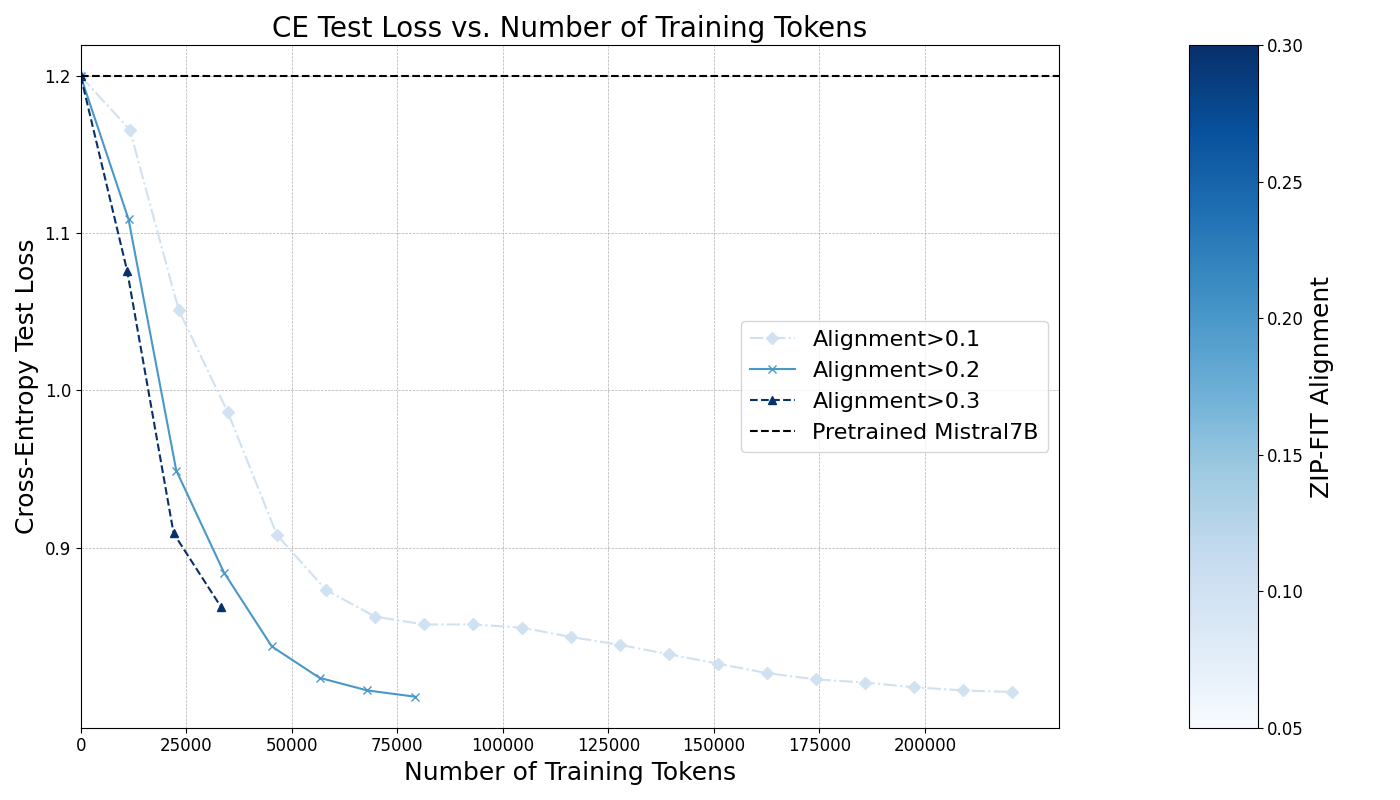
\includegraphics[width=1\textwidth]{./plots/remove_misaligned_data2.png}}
  \caption{\textbf{Selective data filtering with \texttt{ZIP-FIT} allows us to achieve better cross-entropy test loss faster than training on all the data, resulting in improved performance and efficiency.} 
  The x-axis represents the number of training tokens, while the y-axis shows the cross-entropy test loss. 
  The curves represent models fine-tuned (FT) on datasets filtered by varying alignment thresholds ($>$ 0.1, $>$ 0.2, $>$ 0.3).
  The dashed line indicates the baseline performance of the pretrained Mistral7B model. 
  Training on data filtered with higher alignment thresholds leads to superior performance, demonstrating the effectiveness of removing misaligned data in fine-tuning.
  }
  \label{fig:misaligned-data}
\end{figure*}
